\documentclass{article}
\usepackage[utf8]{inputenc}
\usepackage{amsmath}
\usepackage{amsfonts}
\usepackage{tikz}

\begin{document}

\thispagestyle{empty}

\begin{figure}[htbp]
\centering
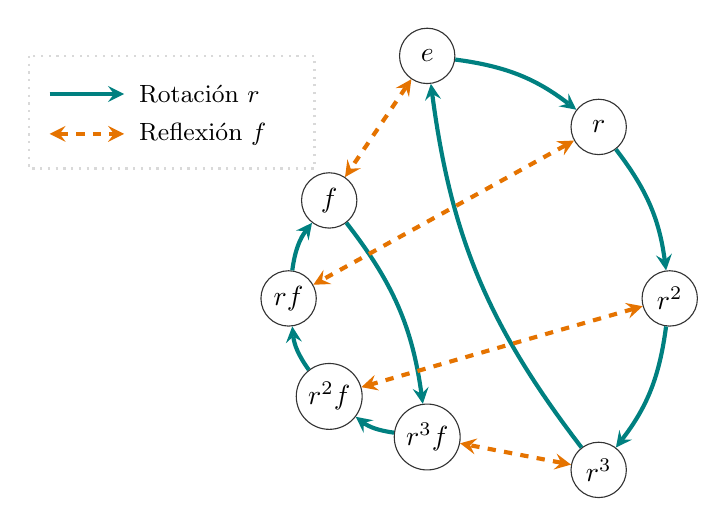
\begin{tikzpicture}[
    scale=2.2,
    % --- NODOS: Letra en \normalsize y espacio interior adecuado ---
    nodo/.style={circle, draw=black!80, fill=white, inner sep=2pt, minimum size=2em, font=\normalsize},
    % --- ARISTAS: Grosor ajustado a 1.5pt ---
    flechaRotacion/.style={->, >=stealth, color=teal, line width=1.5pt},
    flechaReflexion/.style={<->, >=stealth, color=orange!90!black, dashed, line width=1.5pt}
]

    % --- DEFINICIÓN DE LOS 8 VÉRTICES ---
    % Rotaciones (Círculo exterior)
    \node[nodo] (e)   at (90:1.4)   {$e$};
    \node[nodo] (r)   at (45:1.4)   {$r$};
    \node[nodo] (r2)  at (0:1.4)    {$r^2$};
    \node[nodo] (r3)  at (315:1.4)  {$r^3$};
    
    % Reflexiones combinadas (Círculo interior)
    \node[nodo] (f)   at (135:0.8)  {$f$};
    \node[nodo] (rf)  at (180:0.8)  {$rf$};
    \node[nodo] (r2f) at (225:0.8)  {$r^2f$};
    \node[nodo] (r3f) at (270:0.8)  {$r^3f$};


    % --- ARISTAS DEL GENERADOR 'r' ---
    \draw[flechaRotacion] (e) to[bend left=15] (r);
    \draw[flechaRotacion] (r) to[bend left=15] (r2);
    \draw[flechaRotacion] (r2) to[bend left=15] (r3);
    \draw[flechaRotacion] (r3) to[bend left=15] (e);

    \draw[flechaRotacion] (f) to[bend left=15] (r3f);
    \draw[flechaRotacion] (r3f) to[bend left=15] (r2f);
    \draw[flechaRotacion] (r2f) to[bend left=15] (rf);
    \draw[flechaRotacion] (rf) to[bend left=15] (f);


    % --- ARISTAS DEL GENERADOR 'f' ---
    \draw[flechaReflexion] (e) -- (f);
    \draw[flechaReflexion] (r) -- (rf);
    \draw[flechaReflexion] (r2) -- (r2f);
    \draw[flechaReflexion] (r3) -- (r3f);


    % --- LEYENDA INTEGRADA ---
    \begin{scope}[shift={(-2.3,1.4)}]
        \draw[fill=white, draw=gray!30, dotted, thick] (0,0) rectangle (1.65,-0.65);
        \draw[flechaRotacion] (0.12,-0.22) -- (0.55,-0.22);
        \node[right, black, font=\small] at (0.58,-0.22) {Rotación $r$};
        
        \draw[flechaReflexion] (0.12,-0.45) -- (0.55,-0.45);
        \node[right, black, font=\small] at (0.58,-0.45) {Reflexión $f$};
    \end{scope}

\end{tikzpicture}

\end{figure}

\end{document}
